\documentclass[aspectratio=169,kulak,t,handout]{kulakbeamer} % handout

\usepackage[dutch]{babel}
\usepackage[T1]{fontenc}
\usefonttheme[onlymath]{serif}

\title[Beamer]{Miniatuur Robotwagen in een Smart City}

\author{Camille Louagie, Emile Vanspranghels, Otto Meerschman, Ruben Leenknecht, Staf Rys} 
\institute[Kulak]{KU Leuven Kulak}
\date{Academiejaar 2020 -- 2021}

\AtBeginSection[]{\only<beamer>{\addtocounter{framenumber}{-1}
		\begin{outlineframe}\frametitle{Overzicht}
			\tableofcontents[currentsection,hideallsubsections]
	\end{outlineframe}}}


\begin{document}

\begin{titleframe}
\titlepage
\end{titleframe}

\begin{outlineframe}[Overzicht]
\tableofcontents
\end{outlineframe}

\section{Inleiding}

\begin{frame}
	\frametitle{Nood aan efficiëntie}
	\begin{itemize}
		\item  Maatschappelijke uitdagingen
		\begin{itemize}
			\item Toename verstedelijking
			\item Verscheidene problemen
			\item Technologie
		\end{itemize}
		\item Slimme steden als oplossing
	\end{itemize}
	
	\begin{figure}
		\centering
		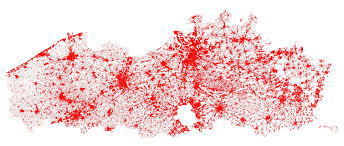
\includegraphics[width=.60\textwidth]{ruimtelijkestaat}
		%rood= ruimtebeslag > drempelwaarde
		
		\label{fig:CAD-model}
	\end{figure}
	
\end{frame}

\begin{frame}
	\frametitle{Smart Cities}
	
\begin{block}{Definitie}
	
	Een stad die technologische innovatie gebruikt om de stedelijke werking efficiënt te laten verlopen
	
\end{block}	
	\begin{itemize}
		\item  Verbeteren van interacties
		\begin{itemize}
			\item Fysieke beperkingen
			\item Levenskwaliteit verhogen
		\end{itemize}
		\item  Diensten vereenvoudigen
	\end{itemize}



\end{frame}

\begin{frame}{Zelfrijdende Auto's}
	\begin{columns}
	\column{0.5\textwidth}\centering
	{\bf{Voordelen}}\\[.2cm]

		\begin{itemize}
			\item Rijden nauwkeuriger
			\begin{itemize}
				\item Meer parkeerplaatsen
				\item Minder files
			\end{itemize}
			\item Respect voor verkeersregels
			
		\end{itemize}
	\column{0.5\textwidth}\centering
	{\bf{Nadelen}}\\[.2cm]

			\begin{itemize}
			\item Kwetsbaar voor hackers
			\item Verminderde inkomst overheid
			\item Stijging werkeloosheid
			\end{itemize}
	
	\end{columns}
\end{frame}

\section{Ontwerp}

\begin{frame}{Ontwerp}
	\begin{columns}
		\begin{column}{0.47\textwidth}\centering
			{\bf{Onderdelen}}\\[.2cm]
			\begin{itemize}
				\item Microcontroller
				\item Motor
				\item Sensoren
				\item Batterij
				\item Wielen
				\item Chassis
			\end{itemize}
		\end{column}
		\begin{column}{0.75\textwidth}\centering
		{\bf{CAD-model}}\\[.2cm]
			\begin{figure}
				\centering
				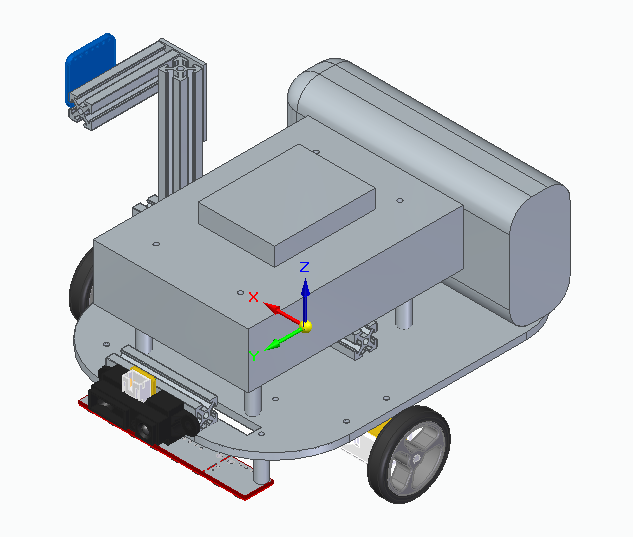
\includegraphics[width=.60\textwidth]{afbchassis}
				
				\label{fig:CAD-model}
			\end{figure}
		\end{column}
	\end{columns}
\end{frame}

\begin{frame}{Chassis}
	\begin{columns}
	\begin{column}{0.50\textwidth}\centering
		%{\bf{Onderdelen}}\\[.2cm]
		\begin{itemize}
			\item Afmetingen
			\item Hoek met de grond
			\item Lijnsensor
			\item Ball Caster
			\item Wielen
		\end{itemize}
	\end{column}
	\begin{column}{0.75\textwidth}\centering
		{\bf{Chassis-model}}\\[.2cm]
		\begin{figure}
			\centering
			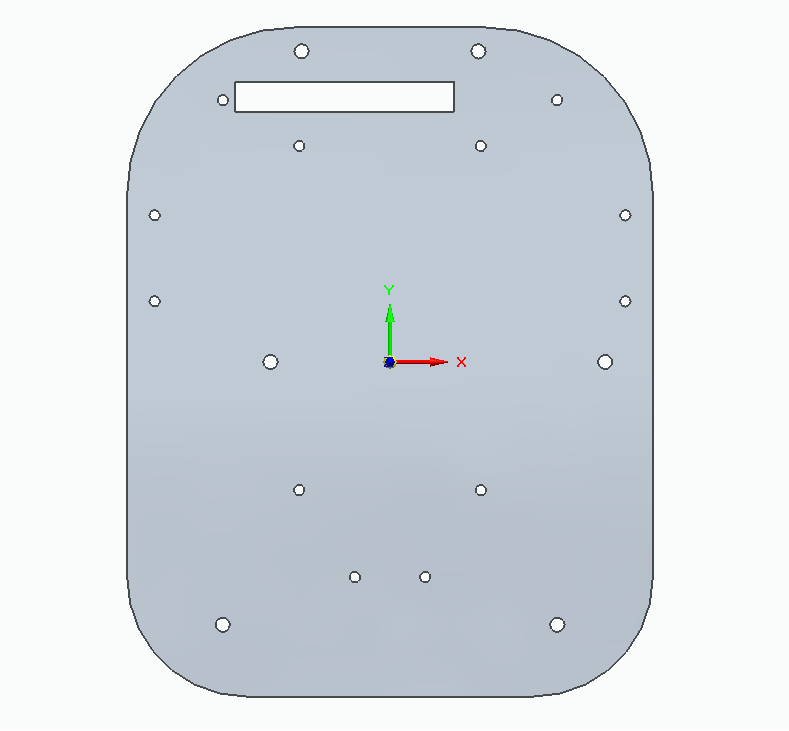
\includegraphics[width=.55\textwidth]{chassis3d}
			
			\label{fig:chassis}
		\end{figure}
	\end{column}
\end{columns}	
\end{frame}

\end{document}